% !TEX program = pdflatex
\documentclass[final]{beamer}
\usepackage{filecontents}

\begin{filecontents*}[overwrite]{beamerposter.sty}
% ============================================================
% beamerposter.sty  –  Beamer Poster Extension (v1.07)
% Original: Philippe Dreuw & Thomas Deselaers, 2007–2008
% Kommentiert & optimiert für einfache Anpassung
% ============================================================

\def\beamerposter@version{1.07}
\def\beamerposter@date{2008/03/11}
\def\beamerposter@msg{beamerposter: latex-beamer poster extension}
\typeout{Package: \beamerposter@date. v.\beamerposter@version. \beamerposter@msg}

\NeedsTeXFormat{LaTeX2e}
\ProvidesPackage{beamerposter}[\beamerposter@date. v.\beamerposter@version. \beamerposter@msg]
\RequirePackage{xkeyval}[2006/11/18]
\RequirePackage{type1cm}   % skalierbare Mathe-Fonts (Type1)

% ============================================================
% INTERNE FLAGS  (nicht ändern)
% ============================================================
\newif\ifportrait    % wird durch Option orientation=portrait gesetzt
\newif\ifcustomsize  % wird durch Option size=custom gesetzt
\newif\ifdebug       % aktiviert Debug-Ausgaben

% ============================================================
% PAKET-OPTIONEN  –  werden beim \usepackage gesetzt
% ============================================================
% Verwendung im Dokument:
%   \usepackage[size=a0, orientation=portrait, scale=1.4]{beamerposter}
%
% ┌─────────────────────────────────────────────────────────┐
% │  OPTION: size                                           │
% │  Werte:  a0b | a0 | a1 | a2 | a3 | a4 | custom          │
% │  → custom erfordert zusätzlich width=… und height=…    │
% └─────────────────────────────────────────────────────────┘
\DeclareOptionX{size}[a0]{
  \typeout{beamerposter: checking size input, please wait.}
  \XKV@cc*+[\val\nr]{#1}{a0b,a0,a1,a2,a3,a4,custom}{%
    \typeout{beamerposter: the input \val\ \nr\ was correct, we proceed.}
    \ifcase\nr\relax

    % ----- a0b (etwas größer als DIN A0, für ältere Drucker) -----
    \setlength{\paperheight}{119cm}
    \setlength{\paperwidth} {88cm}
    \setlength{\textheight} {116cm}
    \setlength{\textwidth}  {88cm}
    \or

    % ----- a0  (Standard DIN A0 – empfohlen!) --------------------
    \setlength{\paperheight}{118.82cm}
    \setlength{\paperwidth} {83.96cm}
    \setlength{\textheight} {117.82cm}
    \setlength{\textwidth}  {82.96cm}
    \or

    % ----- a1 ----------------------------------------------------
    \setlength{\paperheight}{83.96cm}
    \setlength{\paperwidth} {59.4cm}
    \setlength{\textheight} {82.96cm}
    \setlength{\textwidth}  {58.4cm}
    \or

    % ----- a2 ----------------------------------------------------
    \setlength{\paperheight}{59.4cm}
    \setlength{\paperwidth} {41.98cm}
    \setlength{\textheight} {58.4cm}
    \setlength{\textwidth}  {40.98cm}
    \or

    % ----- a3 ----------------------------------------------------
    \setlength{\paperwidth} {41.98cm}
    \setlength{\paperheight}{29.7cm}
    \setlength{\textwidth}  {40.98cm}
    \setlength{\textheight}{28.7cm}
    \or

    % ----- a4 ----------------------------------------------------
    \setlength{\paperheight}{29.7cm}
    \setlength{\paperwidth} {21.0cm}
    \setlength{\textheight} {28.7cm}
    \setlength{\textwidth}  {20.0cm}
    \or

    % ----- custom  (eigene Maße via width= und height=) ----------
    \customsizetrue
    \fi
  }{%
    \PackageWarning{beamerposter}{the input \val\ was incorrect and was ignored.}
  }%
  \typeout{beamerposter: finished size input check.}
}

% ┌─────────────────────────────────────────────────────────┐
% │  OPTION: orientation                                    │
% │  Werte:  portrait (Hochformat) | landscape (Querformat) │
% │  → tauscht paperwidth ↔ paperheight                    │
% └─────────────────────────────────────────────────────────┘
\DeclareOptionX{orientation}[portrait]{
  \typeout{beamerposter: checking orientation input, please wait.}
  \XKV@cc*+[\val\nr]{#1}{portrait,landscape}{%
    \typeout{beamerposter: the input \val\ \nr\ was correct, we proceed.}
    \ifcase\nr\relax
      \portraittrue   % Hochformat
    \or
      \portraitfalse  % Querformat
    \fi
  }{%
    \PackageWarning{beamerposter}{the input \val\ was incorrect and was ignored.}
  }%
  \typeout{beamerposter: finished orientation check.}
}

% ┌─────────────────────────────────────────────────────────┐
% │  OPTION: scale                                          │
% │  Wert:  Dezimalzahl, z. B. 1.0 / 1.2 / 1.4 / 1.5        │
% │  → skaliert ALLE Schriftgrößen gleichmäßig             │
% │  Tipp: 1.4 ist ein guter Startpunkt für A0-Poster       │
% └─────────────────────────────────────────────────────────┘
\DeclareOptionX{scale}[1.0]{%
  \edef\myfontscale{#1}%
  \typeout{beamerposter: myfontscale=\myfontscale}%
}

% ┌─────────────────────────────────────────────────────────┐
% │  OPTIONEN: width / height  (nur bei size=custom)        │
% │  Wert:  Zahl in cm, z. B.  width=120  height=90         │
% └─────────────────────────────────────────────────────────┘
\DeclareOptionX{width} {\edef\customwidth{#1} \typeout{beamerposter: custom width=\customwidth}}
\DeclareOptionX{height}{\edef\customheight{#1}\typeout{beamerposter: custom height=\customheight}}

% ┌─────────────────────────────────────────────────────────┐
% │  OPTION: debug                                          │
% │  → gibt Seitenmaße als \typeout aus; nützlich beim      │
% │    Entwickeln / Debuggen                                │
% └─────────────────────────────────────────────────────────┘
\DeclareOptionX{debug}{\typeout{beamerposter: enabled debug mode}\debugtrue}

\DeclareOptionX*{\PackageWarning{beamerposter}{Unknown option ignored: \CurrentOption}}

% Standard-Optionen (wenn nichts angegeben wird):
\ExecuteOptionsX{size=a0, scale=1.0}
\ProcessOptionsX\relax

% ============================================================
% FP-PAKET  (Fließkomma-Arithmetik für Schriftgrößen)
% ============================================================
\ifdebug
  \RequirePackage[debug]{fp}
\else
  \RequirePackage{fp}
\fi

% ============================================================
% ORIENTIERUNG  –  Maße bei portrait tauschen
% ============================================================
\ifportrait
  \newdimen\tmp
  \setlength{\tmp}{\paperwidth}
  \setlength{\paperwidth}{\paperheight}
  \setlength{\paperheight}{\tmp}
  \setlength{\tmp}{\textwidth}
  \setlength{\textwidth}{\textheight}
  \setlength{\textheight}{\tmp}
\else\relax
\fi

% ============================================================
% CUSTOM SIZE  –  eigene Maße einsetzen
% ============================================================
% Texthöhe/-breite = Papiermaß − 1 cm Rand (fest kodiert)
% → Für mehr Rand hier den FPupn-Ausdruck anpassen,
%   z. B.  {2 customwidth  -}  für 2 cm Rand pro Seite
\ifcustomsize
  \setlength{\paperwidth} {\customwidth cm}
  \setlength{\paperheight}{\customheight cm}
  \FPupn{\resulttextwidth} {1 customwidth  -}
  \FPupn{\resulttextheight}{1 customheight -}
  \setlength{\textwidth} {\resulttextwidth cm}
  \setlength{\textheight}{\resulttextheight cm}
\fi

% ============================================================
% SEITENRÄNDER  –  Feintuning für DIN-A0-Drucker
% ============================================================
% Diese Werte kompensieren LaTeX-interne 1-Zoll-Offsets.
% Nur ändern, wenn der Ausdruck verschoben wirkt!
\setlength{\headheight}  {0 cm}
\setlength{\headsep}     {0 cm}
\setlength{\topmargin}   {-12.7 mm}   % = -1in + 1.47 cm
\setlength{\oddsidemargin}{-25.4 mm}  % = -1in + 0.4 cm

% ┌─────────────────────────────────────────────────────────┐
% │  GEOMETRY  –  hier Rand des Posters anpassen            │
% │  hmargin = linker & rechter Rand                        │
% │  vmargin = oberer & unterer Rand                        │
% │  head/foot = Platz für Kopf-/Fußzeile                  │
% └─────────────────────────────────────────────────────────┘
\ifdebug
  \typeout{beamerposter: paperwidth=\the\paperwidth, paperheight=\the\paperheight}
  \typeout{beamerposter: textwidth=\the\textwidth,   textheight=\the\textheight}
\fi

\geometry{
  paperwidth  = \the\paperwidth,
  paperheight = \the\paperheight,
  hmargin     = 0.12cm,
  vmargin     = 0.12cm,
  head        = 0.12cm,
  headsep     = 0pt,
  foot        = 0.12cm
}

% ============================================================
% SCHRIFTGRÖSSENS-TABELLE
% ============================================================
% Alle Standardbefehle (\tiny … \Huge) werden auf A0-taugliche
% Größen umskaliert.  Schema: Größe × myfontscale = finale pt.
%
% ┌──────────────┬───────────┬──────────────────────────────┐
% │ Befehl       │ Basis-pt  │ Verwendung auf Poster        │
% ├──────────────┼───────────┼──────────────────────────────┤
% │ \tiny        │  14.4 pt  │ Fußnoten, sehr kleiner Text  │
% │ \scriptsize  │  17.3 pt  │ Bildunterschriften           │
% │ \footnotesize│  20.7 pt  │ Referenzen                   │
% │ \small       │  24.9 pt  │ Blockinhalte (kompakt)       │
% │ \normalsize  │  29.9 pt  │ Fließtext  ← Hauptgröße      │
% │ \large       │  35.8 pt  │ Zwischenüberschriften        │
% │ \Large       │  43.0 pt  │ Block-Titel                  │
% │ \LARGE       │  51.6 pt  │ Abschnitts-Überschriften     │
% │ \huge        │  61.9 pt  │ Spalten-Überschriften        │
% │ \semiHuge    │  67.8 pt  │ (neu) Poster-Untertitel      │
% │ \Huge        │  74.3 pt  │ Poster-Titel                 │
% │ \veryHuge    │  80.3 pt  │ (neu) extra groß             │
% │ \VeryHuge    │ 107.0 pt  │ (neu) maximale Größe         │
% └──────────────┴───────────┴──────────────────────────────┘
%
% ERWEITERUNG: Neue Größe hinzufügen →  Muster kopieren:
%   \edef\fontSizeX{XX.X}\edef\fontSizeY{YY}          % pt / Zeilenabstand
%   \FPupn{\resultMeineGroesseX}{myfontscale fontSizeX * 2 round}
%   \FPupn{\resultMeineGroesseY}{myfontscale fontSizeY * 2 round}
%   \newcommand*{\meineGroesse}{\fontsize{\resultMeineGroesseX}{\resultMeineGroesseY}\selectfont}

% --- \tiny ---------------------------------------------------
\edef\fontSizeX{14.4}\edef\fontSizeY{18}
\FPupn{\resultscriptsizeX}{myfontscale fontSizeX * 2 round}
\FPupn{\resultscriptsizeY}{myfontscale fontSizeY * 2 round}
\renewcommand*{\tiny}{\fontsize{\resultscriptsizeX}{\resultscriptsizeY}\selectfont}

% --- \scriptsize ---------------------------------------------
\edef\fontSizeX{17.28}\edef\fontSizeY{22}
\FPupn{\resultfootnotesizeX}{myfontscale fontSizeX * 2 round}
\FPupn{\resultfootnotesizeY}{myfontscale fontSizeY * 2 round}
\renewcommand*{\scriptsize}{\fontsize{\resultfootnotesizeX}{\resultfootnotesizeY}\selectfont}

% --- \footnotesize -------------------------------------------
\edef\fontSizeX{20.74}\edef\fontSizeY{25}
\FPupn{\resultsmallX}{myfontscale fontSizeX * 2 round}
\FPupn{\resultsmallY}{myfontscale fontSizeY * 2 round}
\renewcommand*{\footnotesize}{\fontsize{\resultsmallX}{\resultsmallY}\selectfont}

% --- \small --------------------------------------------------
\edef\fontSizeX{24.88}\edef\fontSizeY{30}
\FPupn{\resultnormalsizeX}{myfontscale fontSizeX * 2 round}
\FPupn{\resultnormalsizeY}{myfontscale fontSizeY * 2 round}
\renewcommand*{\small}{\fontsize{\resultnormalsizeX}{\resultnormalsizeY}\selectfont}

% --- \normalsize  ← HAUPTTEXTGRÖSSE --------------------------
\edef\fontSizeX{29.86}\edef\fontSizeY{37}
\FPupn{\resultlargeX}{myfontscale fontSizeX * 2 round}
\FPupn{\resultlargeY}{myfontscale fontSizeY * 2 round}
\renewcommand*{\normalsize}{\fontsize{\resultlargeX}{\resultlargeY}\selectfont}

% --- \large --------------------------------------------------
\edef\fontSizeX{35.83}\edef\fontSizeY{45}
\FPupn{\resultLargeX}{myfontscale fontSizeX * 2 round}
\FPupn{\resultLargeY}{myfontscale fontSizeY * 2 round}
\renewcommand*{\large}{\fontsize{\resultLargeX}{\resultLargeY}\selectfont}

% --- \Large --------------------------------------------------
\edef\fontSizeX{43}\edef\fontSizeY{54}
\FPupn{\resultLARGEX}{myfontscale fontSizeX * 2 round}
\FPupn{\resultLARGEY}{myfontscale fontSizeY * 2 round}
\renewcommand*{\Large}{\fontsize{\resultLARGEX}{\resultLARGEY}\selectfont}

% --- \LARGE --------------------------------------------------
\edef\fontSizeX{51.6}\edef\fontSizeY{64}
\FPupn{\resulthugeX}{myfontscale fontSizeX * 2 round}
\FPupn{\resulthugeY}{myfontscale fontSizeY * 2 round}
\renewcommand*{\LARGE}{\fontsize{\resulthugeX}{\resulthugeY}\selectfont}

% --- \huge ---------------------------------------------------
\edef\fontSizeX{61.92}\edef\fontSizeY{77}
\FPupn{\resultHugeX}{myfontscale fontSizeX * 2 round}
\FPupn{\resultHugeY}{myfontscale fontSizeY * 2 round}
\renewcommand*{\huge}{\fontsize{\resultHugeX}{\resultHugeY}\selectfont}

% --- \semiHuge  (neu, kein Standard-LaTeX) -------------------
\edef\fontSizeX{67.8}\edef\fontSizeY{84.6}
\FPupn{\resultsemiHugeX}{myfontscale fontSizeX * 2 round}
\FPupn{\resultsemiHugeY}{myfontscale fontSizeY * 2 round}
\newcommand*{\semiHuge}{\fontsize{\resultsemiHugeX}{\resultsemiHugeY}\selectfont}

% --- \Huge ---------------------------------------------------
\edef\fontSizeX{74.3}\edef\fontSizeY{93}
\FPupn{\resultveryHugeX}{myfontscale fontSizeX * 2 round}
\FPupn{\resultveryHugeY}{myfontscale fontSizeY * 2 round}
\renewcommand*{\Huge}{\fontsize{\resultveryHugeX}{\resultveryHugeY}\selectfont}

% --- \veryHuge  (neu) ----------------------------------------
\edef\fontSizeX{80.3}\edef\fontSizeY{101}
\FPupn{\resultVeryHugeX}{myfontscale fontSizeX * 2 round}
\FPupn{\resultVeryHugeY}{myfontscale fontSizeY * 2 round}
\newcommand*{\veryHuge}{\fontsize{\resultVeryHugeX}{\resultVeryHugeY}\selectfont}

% --- \VeryHuge  (neu, maximale Größe) ------------------------
\edef\fontSizeX{107}\edef\fontSizeY{134}
\FPupn{\resultVERYHugeX}{myfontscale fontSizeX * 2 round}
\FPupn{\resultVERYHugeY}{myfontscale fontSizeY * 2 round}
\newcommand*{\VeryHuge}{\fontsize{\resultVERYHugeX}{\resultVERYHugeY}\selectfont}

% Standard-Schrift auf normalsize zurücksetzen
\renewcommand*{\normalfont}{\normalsize}
\end{filecontents*}

\begin{filecontents*}[overwrite]{beamerthemeWUposter.sty}
% ============================================================
% beamerthemeWUposter.sty  –  A0-Poster-Theme (optimiert)
% ============================================================

\ProvidesPackage{beamerthemeWUposter}

% ------------------------------------------------------------
% PAKETE
% ------------------------------------------------------------
\RequirePackage{tikz}
\usetikzlibrary{arrows,backgrounds}
\RequirePackage[most]{tcolorbox}
\RequirePackage[T1]{fontenc}
\RequirePackage{lmodern}
\RequirePackage{textcomp}
\RequirePackage{amsmath,amssymb}
\usefonttheme{professionalfonts}
\usepackage{ragged2e}     % Für \justifying in Blöcken

% ------------------------------------------------------------
% LISTENABSTÄNDE  –  mehr Luft vor Listen und zwischen Items
% ------------------------------------------------------------
\makeatletter
\def\@listi{%
  \leftmargin\leftmarginii
  \topsep    1ex   % Abstand VOR der Liste
  \parsep    0\p@ \@plus\p@
  \itemsep   4pt}  % Abstand ZWISCHEN Items
\makeatother

% Bildunterschriften-Fix (Nummerierung korrekt anzeigen)
\usecaptiontemplate{%
  \small\structure{\insertcaptionname~\insertcaptionnumber: }\insertcaption}

% ============================================================
% FARBEN
% ============================================================

% --- Kern-Posterfarben (hier Themefarbe anpassen!) ----------
% → \themecolor steuert Titelfarbe, Items, Block-Titel usw.
%   Einfach eine andere Farbe einsetzen, z. B. \definecolor{themecolor}{RGB}{0,70,173}
\definecolor{themecolor}{RGB}{20,66,129}   % Standard: Dunkelblau (dblue)

\definecolor{blackWU}{RGB}{0,0,0}
\definecolor{lgreen} {RGB}{180,210,100}
\definecolor{dblue}  {RGB}{20,66,129}
\definecolor{ddblue} {RGB}{11,36,69}
\definecolor{lred}   {RGB}{220,0,0}
\definecolor{nblue}  {RGB}{28,130,185}
\definecolor{jblue}  {RGB}{20,50,100}

% (Weitere Farben werden nur bei Bedarf in den Folien genutzt –
%  vollständige Liste im Original behalten, hier gekürzt)

% ============================================================
% BEAMER-FARBEN  –  Struktur des Posters
% ============================================================

% Grundpalette (Rahmen, Navigationsleiste – bei Postern meist irrelevant)
\setbeamercolor{palette primary}   {fg=black,bg=white}
\setbeamercolor{palette secondary} {fg=black,bg=white}
\setbeamercolor{palette tertiary}  {bg=black,fg=white}
\setbeamercolor{palette quaternary}{fg=black,bg=white}
\setbeamercolor{structure}         {fg=black}
\setbeamercolor{frametitle}        {bg=black!10,fg=black}

% Items / Aufzählungen
\setbeamercolor{item}          {fg=themecolor}
\setbeamercolor{item projected}{fg=white,bg=themecolor}

% Normale Blöcke (Titel + Inhalt)
\setbeamercolor{block title}{fg=themecolor,bg=white}
\setbeamercolor{block body} {fg=blackWU,  bg=white}

% Alert-Blöcke (umrahmte Blöcke mit grauem Hintergrund)
\setbeamercolor{block alerted title}{fg=themecolor,bg=white}
\setbeamercolor{block alerted body} {fg=blackWU,bg=blackWU!8}

% Literaturverzeichnis
\setbeamercolor{bibliography item}        {fg=blackWU,bg=white}
\setbeamercolor{bibliography entry author}{fg=blackWU,bg=white}

% ============================================================
% SCHRIFTEN
% ============================================================
\setbeamerfont{section in head/foot}  {series=\bfseries}
\setbeamerfont{block title}           {series=\bfseries,size=\Large}
\setbeamerfont{block alerted title}   {series=\bfseries,size=\Large}
\setbeamerfont{frametitle}            {series=\bfseries,size=\large}
\setbeamerfont{block body}            {series=\rmfamily,size=\normalsize}

% ============================================================
% BEAMER-OPTIONEN  (allgemein)
% ============================================================
\setbeamertemplate{title page}[default][colsep=-4bp,rounded=true]
\setbeamertemplate{sections/subsections in toc}[square]
\setbeamertemplate{items}[circle]
\setbeamertemplate{blocks}[width=0.0]
\beamertemplatenavigationsymbolsempty          % keine Navigationsleiste
\setbeamertemplate{bibliography item}[text]

% ============================================================
% KOPFZEILE  –  Poster-Titel, Autoren, Institut
% ============================================================
% Tipp: Das Hintergrundbild / Logo wird typischerweise per
%   \usebackgroundtemplate{\includegraphics[width=\paperwidth]{header_bg.pdf}}
% vor \begin{document} gesetzt.
\setbeamertemplate{headline}{
  \leavevmode
  \begin{columns}
    \begin{column}{0.04\linewidth}\end{column}
    \begin{column}{0.9\linewidth}
      \vskip0.6cm                   % kompakter Kopfbereich
      \raggedright
      % Titel  (Schriftgröße hier anpassen: \Huge / \veryHuge / \VeryHuge)
      \usebeamercolor{title in headline}{%
        \color{blackWU}\Huge\textbf{\inserttitle}\\[1.ex]}
      % Institut / Affiliation
      \usebeamercolor{institute in headline}{%
        \color{blackWU}\large\insertinstitute}
      \vskip0.25cm
    \end{column}
    \begin{column}{0.05\linewidth}\end{column}
  \end{columns}
  \vspace*{-0.25cm}
}

% ============================================================
% BOX-BLOCK  –  kompakte, gerundete Boxen wie in der Vorlage
% ============================================================
% Außen: dezenter grauer Rahmen
% Titel: hellgraue Leiste
% Inhalt: sehr hellgrauer/weißer Hintergrund
\setbeamertemplate{block begin}{
  \par\vskip0.18cm
  \begin{tcolorbox}[
    enhanced,
    width=\linewidth,
    colback=black!2,
    colframe=black!55,
    boxrule=1.4pt,
    arc=4mm,
    outer arc=4mm,
    left=4mm,
    right=4mm,
    top=10mm,
    bottom=3mm,
    boxsep=0mm,
    title=\insertblocktitle,
    colbacktitle=black!16,
    coltitle=black,
    fonttitle=\usebeamerfont{block title},
    lefttitle=4mm,
    righttitle=4mm,
    toptitle=2.5mm,
    bottomtitle=2.5mm,
    titlerule=0pt,
    title filled
  ]
  \usebeamerfont{block body}
  \justifying
}
\setbeamertemplate{block end}{
  \end{tcolorbox}
  \vskip0.08cm
}

% Alert-Blocks verwenden denselben Box-Stil.
\setbeamertemplate{block alerted begin}{
  \par\vskip0.18cm
  \begin{tcolorbox}[
    enhanced,
    width=\linewidth,
    colback=black!6,
    colframe=black!55,
    boxrule=1.4pt,
    arc=4mm,
    outer arc=4mm,
    left=4mm,
    right=4mm,
    top=10mm,           % <--- HIER GEÄNDERT: Abstand nach oben für Fließtext (war 0mm)
    bottom=3mm,
    boxsep=0mm,
    title=\insertblocktitle,
    colbacktitle=black!22,
    coltitle=black,
    fonttitle=\usebeamerfont{block alerted title},
    lefttitle=4mm,
    righttitle=4mm,
    toptitle=2.5mm,
    bottomtitle=2.5mm,
    titlerule=0pt
  ]
  \usebeamerfont{block body}
  \justifying
}
\setbeamertemplate{block alerted end}{
  \end{tcolorbox}
  \vskip0.08cm
}
\end{filecontents*}


% ==========================================================================
% HIER OBEN BLEIBEN DEINE BEIDEN filecontents-BLÖCKE FÜR 
% beamerposter.sty UND beamerthemeWUposter.sty UNVERÄNDERT ERHALTEN!
% ==========================================================================

\usepackage[scale=1.15]{beamerposter}
\usetheme{WUposter}

\usepackage{multicol}
\usepackage{amsmath,amssymb}
\usepackage{xcolor}
\usepackage{setspace}
\usepackage[square,numbers]{natbib}
\bibliographystyle{abbrvnat}
\usepackage{ragged2e}

% --- FARBANPASSUNG AN FRANKFURT UAS ---
\definecolor{frauasblue}{RGB}{0,101,179} % Offizielles Frankfurt UAS Blau
\colorlet{themecolor}{frauasblue}
\setbeamercolor{background canvas}{bg=white}

\logo{\pgfputat{\pgfxy(-12,110)}{\pgfbox[center,base]{
\includegraphics[width=15cm]{docs/FRAUASLogo.pdf}}}}

% Seitenmaße A0 Hochformat
\setlength{\paperwidth}{84.6cm}
\setlength{\paperheight}{119.4cm}

\newlength{\sepmargin}
\newlength{\sepwid}
\newlength{\onecolwid}
% Sehr schmale Außenränder und Spaltenabstände – mehr nutzbare Fläche.
\setlength{\sepmargin}{0.012\paperwidth}
\setlength{\sepwid}{0.012\paperwidth}
\setlength{\onecolwid}{0.481\paperwidth}

% ------------------------------------------------------------------
%  INHALT – nur hier ändern!
% ------------------------------------------------------------------

% --- Kopfzeile ------------------------------------------------
\title{Cloud Computing}
\institute{Allgemeine Informatik - Sommersemester 2026}

% --- Textelemente -----------------------------------------------

\newcommand{\textArchitecture}{
    \textbf{Hardware and Network Architecture}:\\ The cluster contains a Raspberry Pi 5 head node, eight Raspberry Pi 3 worker nodes, and a TP-Link switch\\
    The switch edge ports use STP PortFast to prevent spanning tree delays during network boot
}

\newcommand{\textStorageAndBoot}{
    \textbf{Centralized Storage and Boot Sequence}:\\ The worker nodes perform network boots via local MicroSD cards that exclusively contain the firmware bootcode.bin\\
    The head node uses DHCP, TFTP, and NFS to provide boot files and root filesystems from an external USB storage device\\
    This architecture centralizes storage and eliminates the need for local operating system installations on the worker nodes\\
}

\newcommand{\textAdministration}{
    \textbf{Remote Administration and Security}:\\ The head node routes the internet traffic of the workers via Network Address Translation (NAT)\\
    Tailscale is run on the head node to establish encrypted remote SSH access\\
    This configuration isolates the worker nodes in a private network and prevents public internet sharing\\
}

\newcommand{\textFrontEndBackEnd}{
  \textbf{Backend (Docker Swarm Stack)}:
    FastAPI: REST interface for event processing and node management\\
    PostgreSQL: Relational storage of event and node metadata\\
    SeaweedFS: S3-compatible, distributed object storage for image data\\
    Scalable deployment via manager and worker nodes in the Swarm cluster\\
  
  \vspace{1ex}
  \textbf{Frontend (React Dashboard)}: Central visualization of threat events, camera status, and statistics\\
    Flexible deployment as a Docker container (Nginx) or via Kubernetes (k3s)\\
    API connection to the backend (default port 8000) with a configurable fetch interval\\
}

\newcommand{\textMonitoring}{
    \begin{figure}
        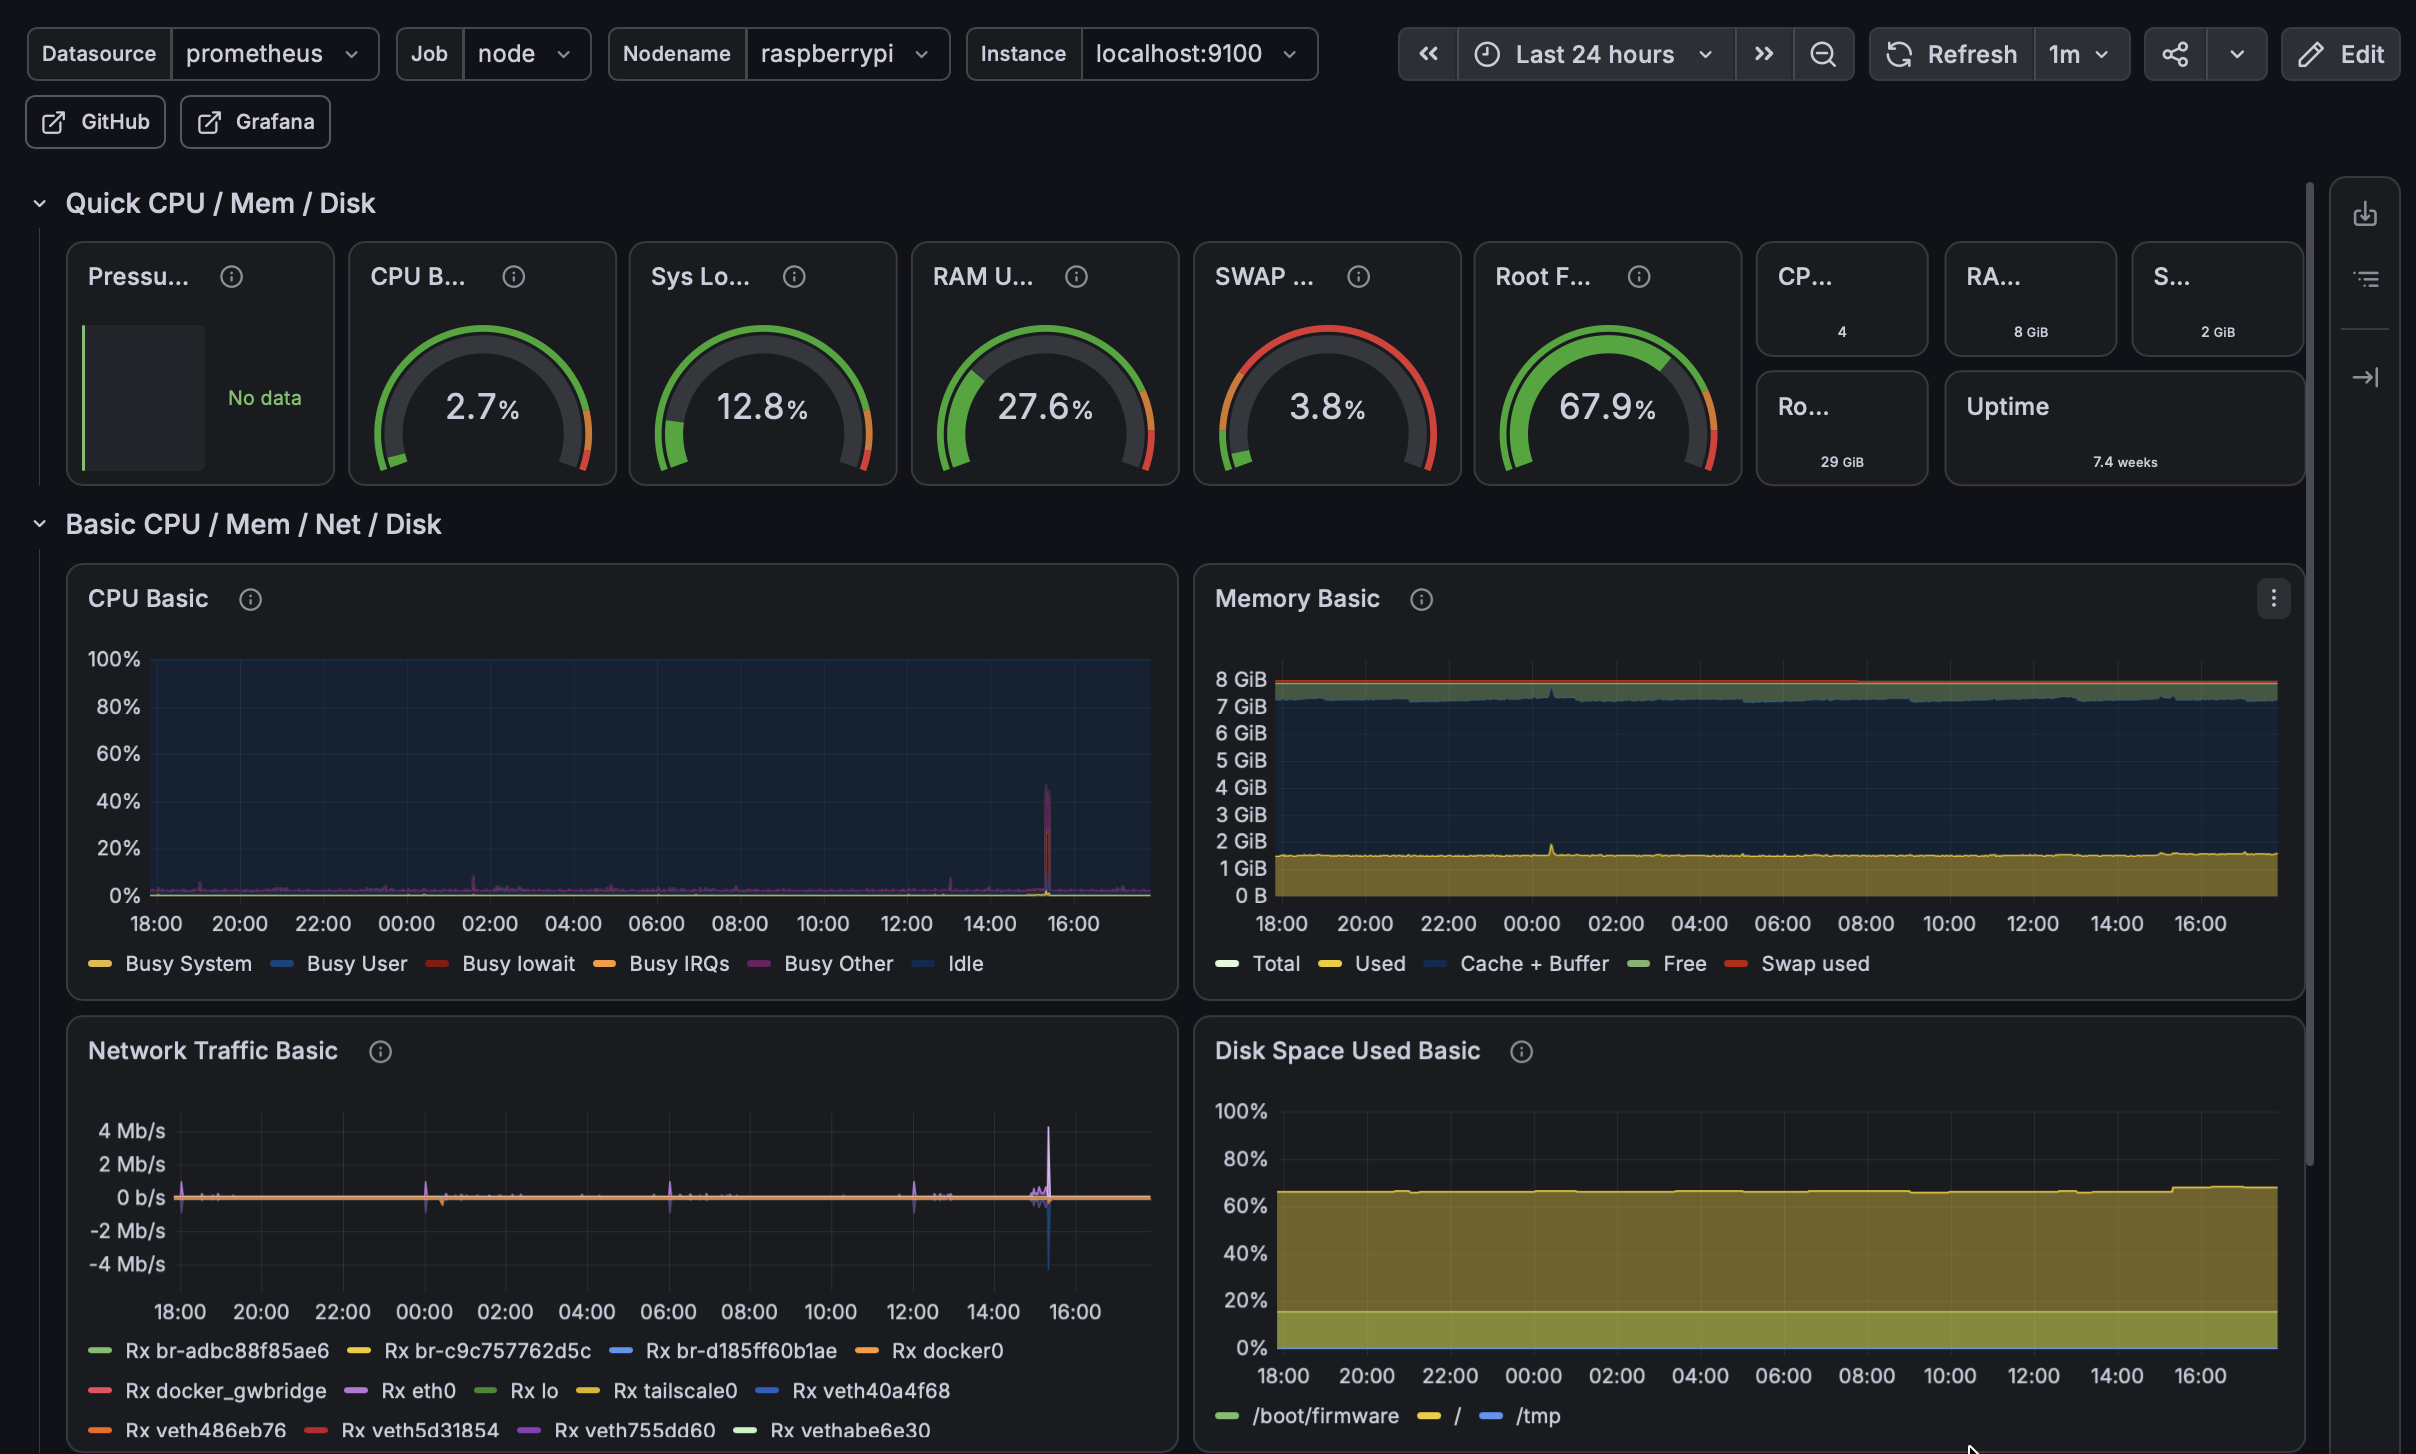
\includegraphics[width=1\linewidth]{docs/monitoring.png}
        \caption{Monitoring}
     \end{figure}
}

\newcommand{\textObjectDetect}{
    \textbf{AI Model \& Architecture:} YOLOv11 (Nano) for real-time edge inference. The project compares two platforms: Raspberry Pi 4 (IMX500 AI Camera) and Raspberry Pi 5 (Hailo-8 AI HAT+)\\
    \textbf{Threat Detection (Classes):} Identification of four specific threats: \textit{Fire}, \textit{Mask}, \textit{Scissors}, and \textit{Knife}\\
    \textbf{Training \& Data (Roboflow):} Custom dataset merged with public datasets, heavily augmented (rotation, brightness, mosaic), and split 70/15/15\\
    \textbf{Deployment 1 (IMX500):} Model exported to \texttt{.imx} via Sony MCT for direct, resource-efficient on-sensor inference\\
    \textbf{Deployment 2 (Hailo-8):} Compilation via ONNX into \texttt{.hef} format for high-performance hardware acceleration\\
    \textbf{Alerting:} Real-time event notifications sent to the backend and integrated with a custom Telegram Bot\\
}

% --- Autoren -------------------------------------------------------
\newcommand{\textContact}{
Yazan Abou Samra, Lorenz Apel, Hicham Chatir, Algis Cinar, Ibrahim El Haj Moussa, Michael Morgenstern, Mohammed Ali Salem Al-Qafeai, Christopher Scheidler Aguilar, Deniz Zimmer \cite{githubrepo}
}
% ------------------------------------------------------------------
%  AB HIER NICHTS ÄNDERN
% ------------------------------------------------------------------

\usepackage{tikz}

\usebackgroundtemplate{
\begin{tikzpicture}[remember picture,overlay]
  \fill[white] (current page.south west) rectangle (current page.north east);
\end{tikzpicture}
}

\begin{document}
  \addtobeamertemplate{block end}{}{\vspace*{1ex}}
  \addtobeamertemplate{block alerted end}{}{\vspace*{0ex}}
  \setlength{\belowcaptionskip}{2ex}

  \begin{frame}[t]
  
    % ===== BREITER BEREICH FÜR TASK 1 (GANZE SEITE) =====
    \begin{columns}[t]
      \begin{column}{\sepmargin}\end{column}
      \begin{column}{\dimexpr\onecolwid+\sepwid+\onecolwid\relax}
        \begin{block}{Architecture}       
          \begin{columns}[T]
            % Text auf der linken Seite des Blocks
            \begin{column}{0.75\linewidth}
              \textArchitecture
              
              \vspace{0.5ex}
              \textStorageAndBoot
              
              \vspace{0.5ex}
              \textAdministration
            \end{column}
            % Bild ganz rechts am Rand des Blocks
            \begin{column}{0.22\linewidth}
              \begin{figure}
                \centering
                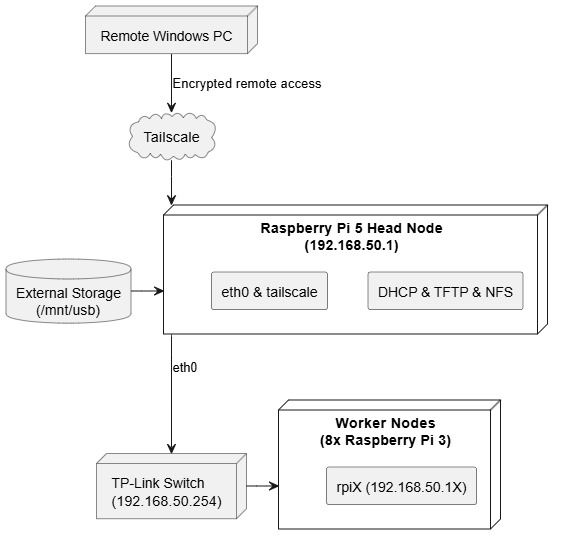
\includegraphics[width=\linewidth]{docs/architecture.jpeg}
                \caption{Architecture \& Remotemanagement}
              \end{figure}
            \end{column}
          \end{columns}
        \end{block}
      \end{column}
      \begin{column}{\sepmargin}\end{column}
    \end{columns}

    \vspace{0.3cm} % Reduzierter Abstand vor den zweispaltigen Inhalten

    % ===== ZWEISPALTIGER BEREICH ==========================
    \begin{columns}[t]
      \begin{column}{\sepmargin}\end{column}

      % ----- LINKE SPALTE -----
      \begin{column}{\onecolwid}
        
        \begin{block}{Frontend \& Backend}
          \textFrontEndBackEnd
        \end{block}

        \begin{block}{Monitoring}
          \textMonitoring
        \end{block}
        
        \begin{block}{Object Detection \& AI Model}
          \textObjectDetect
        \end{block}
        
        % HIER NEU: Authors an die linke Spalte angehängt
        \begin{block}{Authors}
          \begin{footnotesize}
            \textContact
          \end{footnotesize}
        \end{block}
        
      \end{column}

      \begin{column}{\sepwid}\end{column}

      % ----- RECHTE SPALTE -----
      \begin{column}{\onecolwid}
        \begin{block}{Benchmark Results}
          
          \begin{multicols}{2}
          
            % --- LINKE SPALTE (Bilder 1 bis 3) ---
            \begin{figure}
              \vspace*{-0.95cm} 
              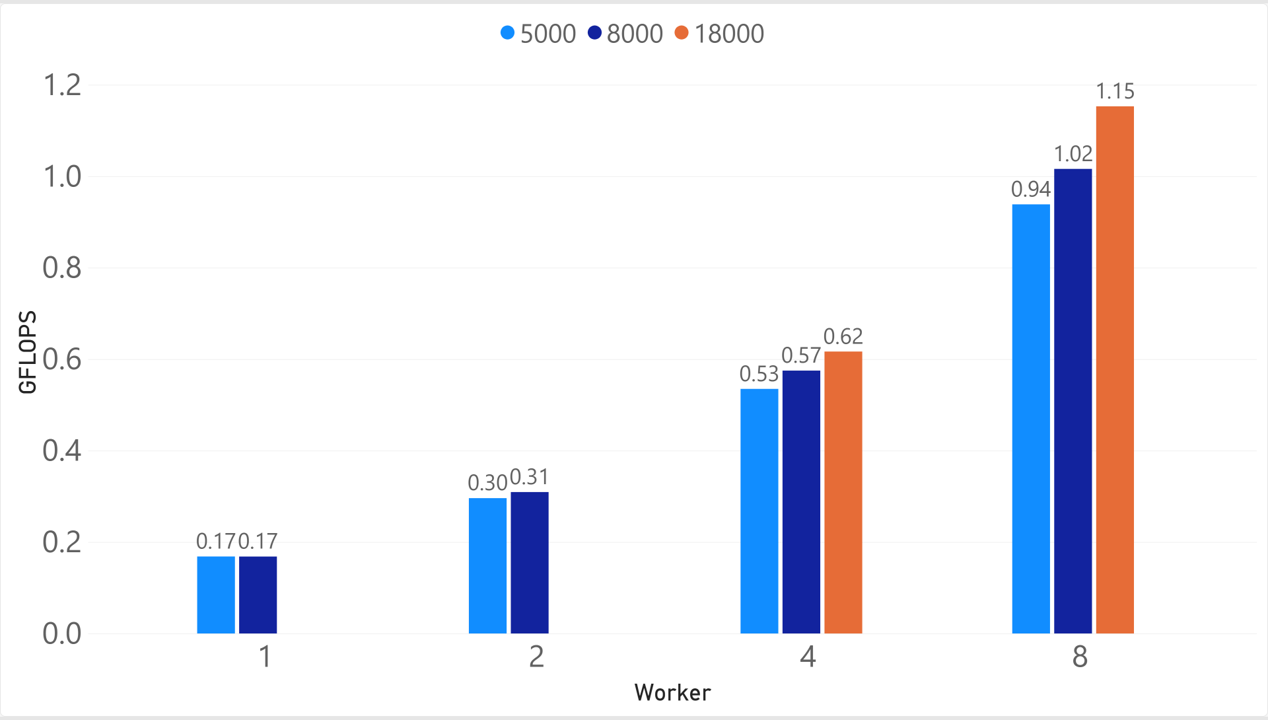
\includegraphics[width=1\linewidth]{docs/HPLLINPACK Performance.png}
              \caption{HPL/LINPACK Performance}
            \end{figure}
            \begin{figure}
              \vspace*{-0.5cm}
              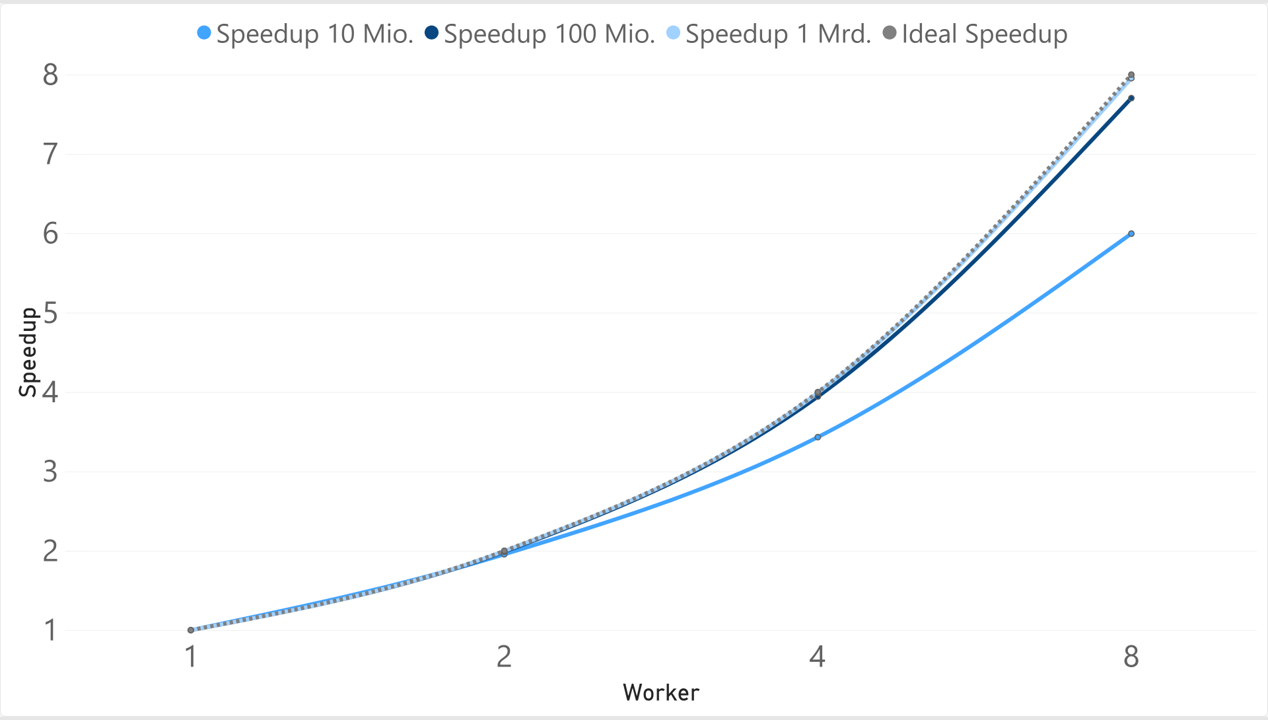
\includegraphics[width=1\linewidth]{docs/Monte Carlo Strong Scaling.png}
              \caption{Monte Carlo Strong Scaling}
            \end{figure}
            \begin{figure}
              \vspace*{-0.5cm}
              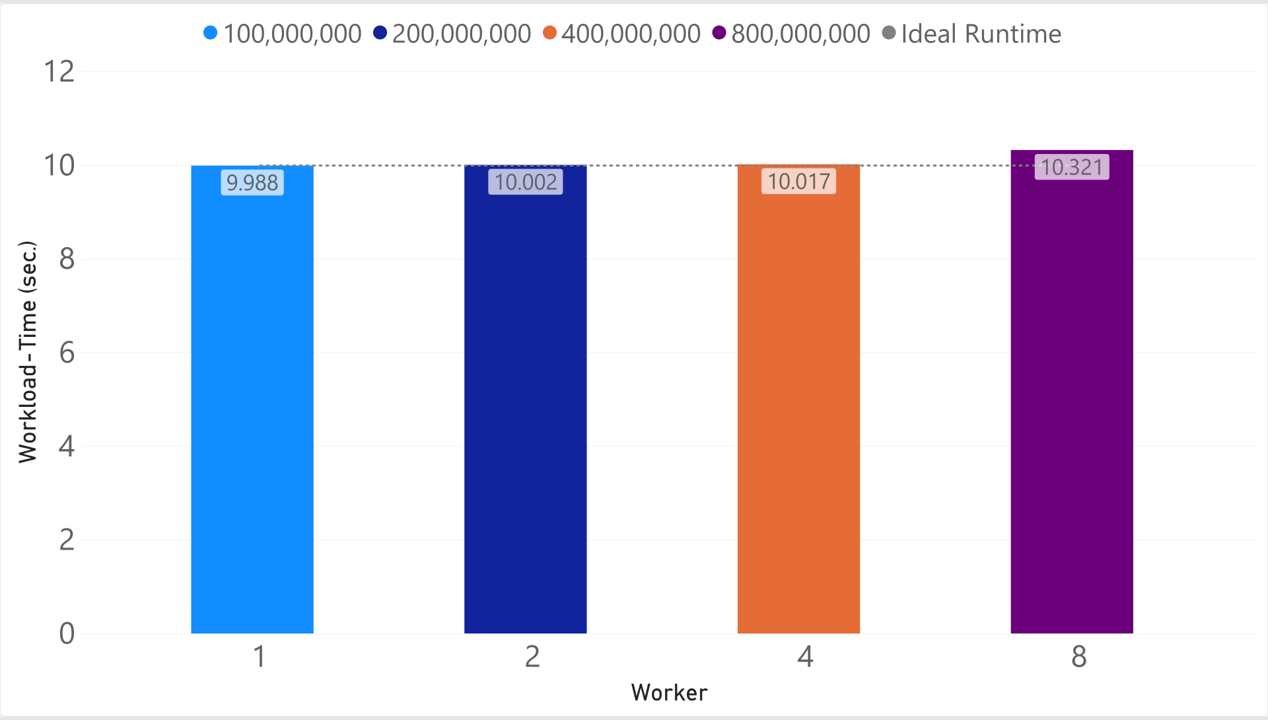
\includegraphics[width=1\linewidth]{docs/Monte Carlo Scaled Workload.png}
              \caption{Monte Carlo Scaled Workload}
            \end{figure}
            
            % --- RECHTE SPALTE (Bilder 4 bis 6) ---
            \begin{figure}
              \vspace*{-0.95cm} 
              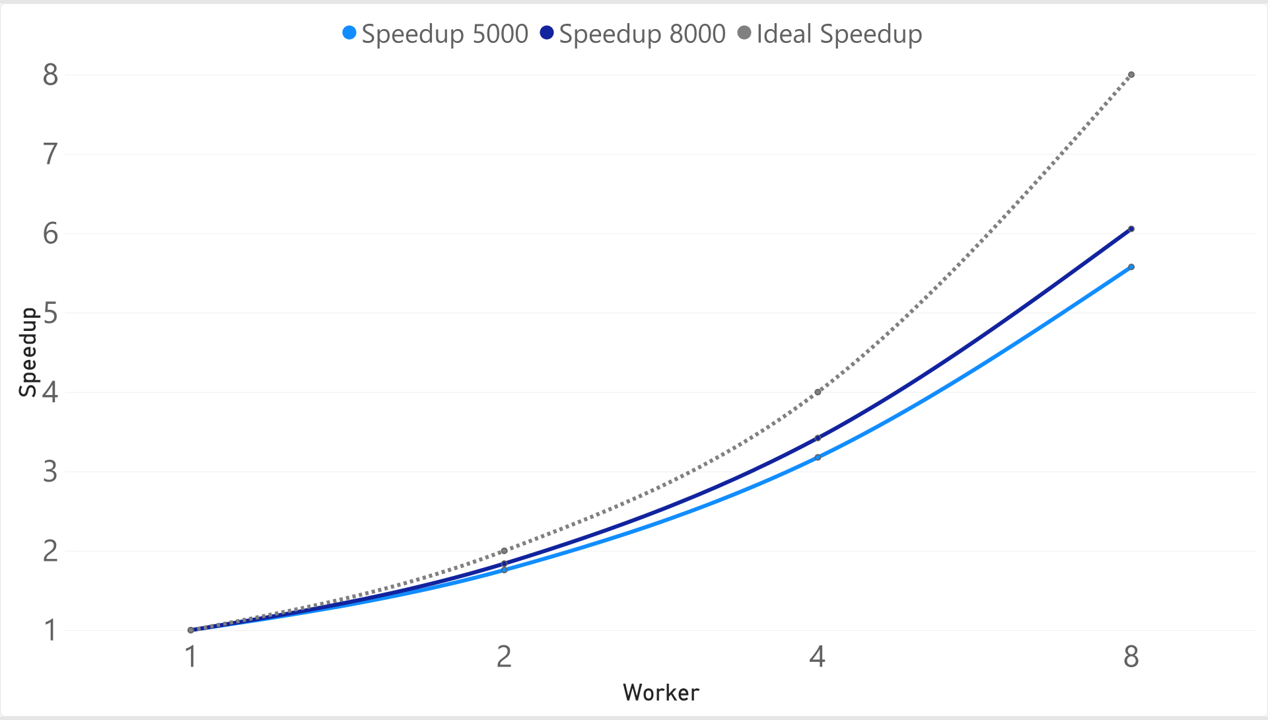
\includegraphics[width=1\linewidth]{docs/HPL Strong Scaling.png}
              \caption{HPL Strong Scaling}
            \end{figure}
            \begin{figure}
              \vspace*{-0.5cm}
              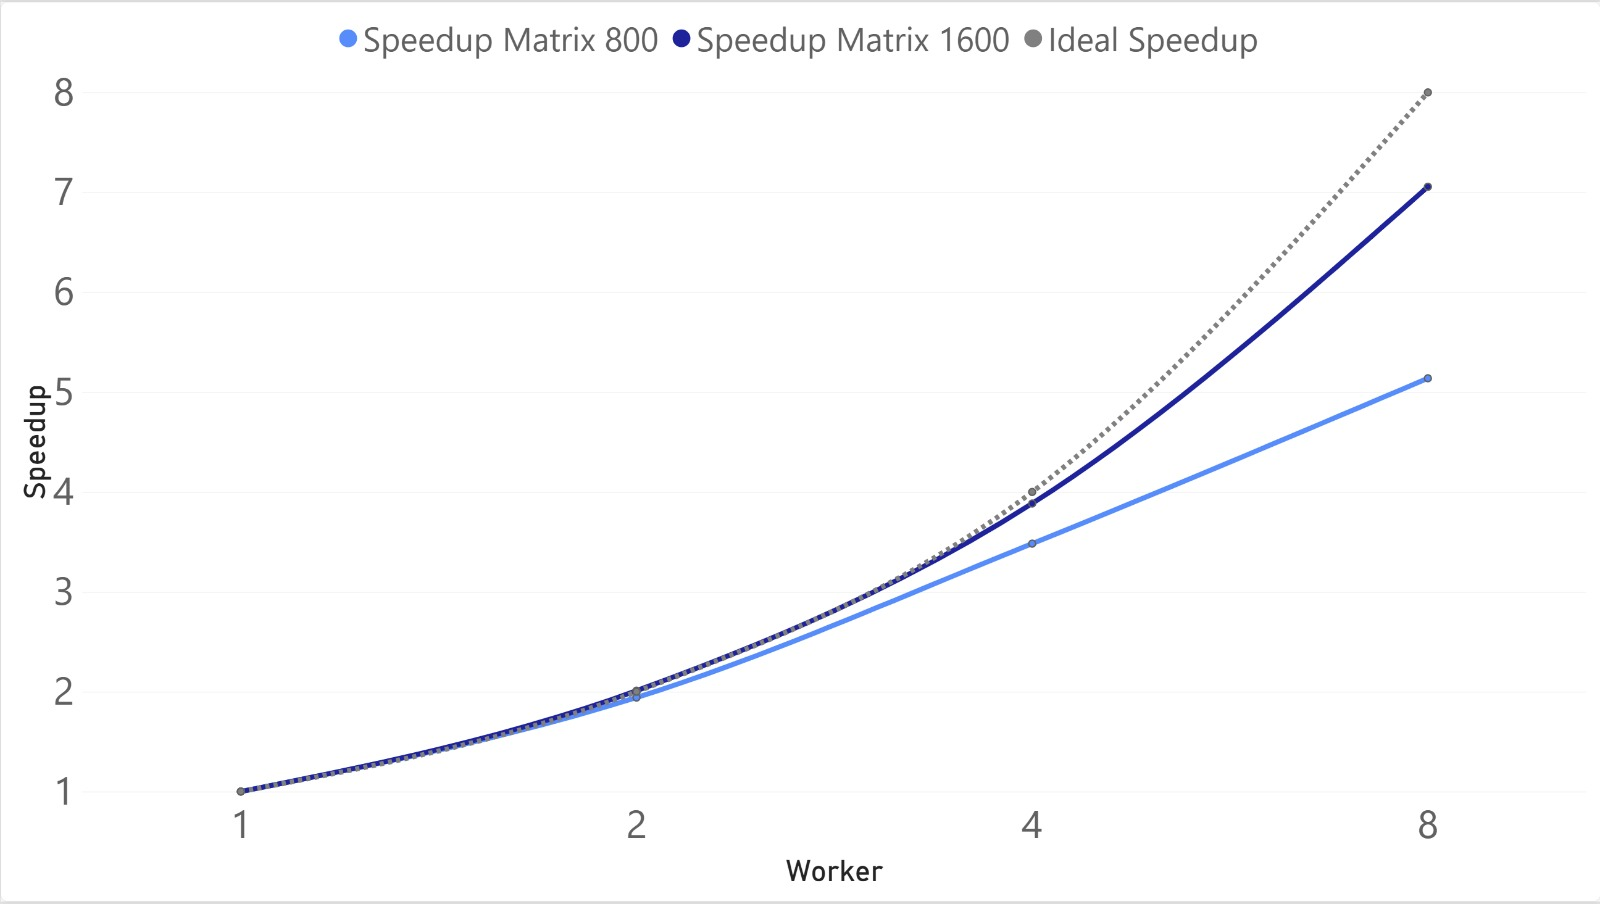
\includegraphics[width=1\linewidth]{docs/Matrix Mulitplication Strong Scaling.jpeg}
              \caption{Matrix Multiplication Strong Scaling}
            \end{figure}
            \begin{figure}
              \vspace*{-0.5cm}
              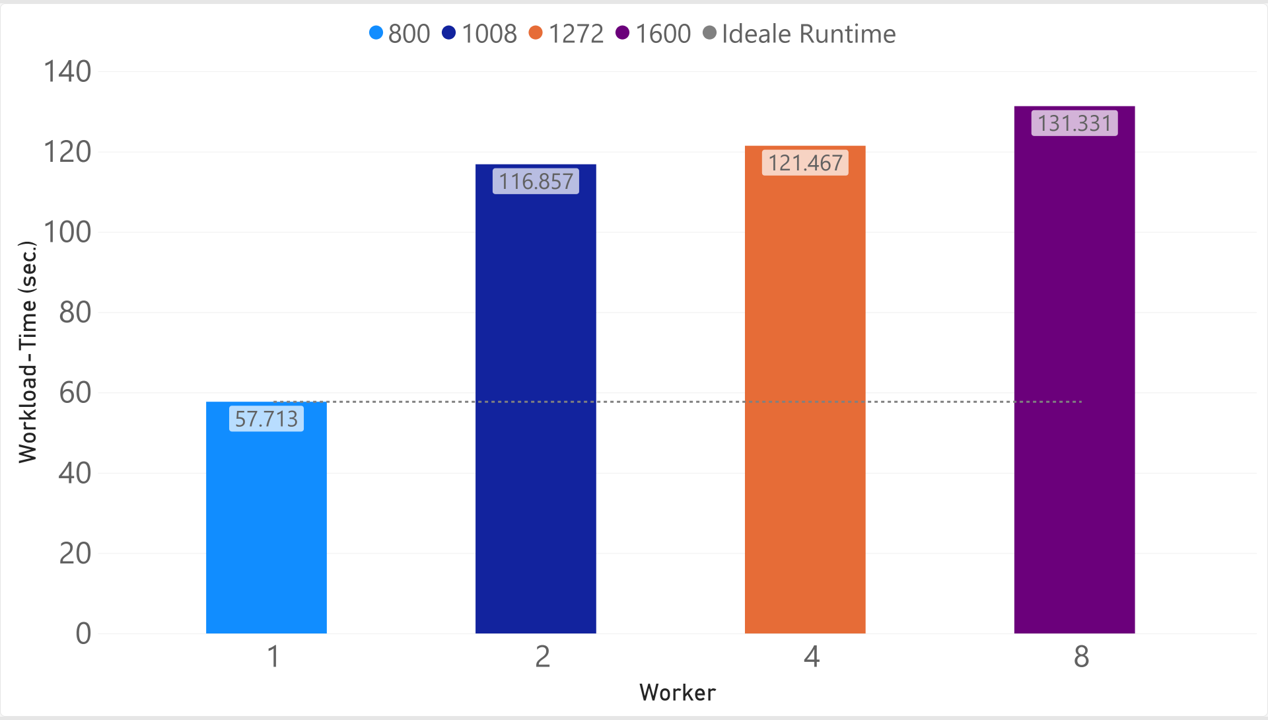
\includegraphics[width=1\linewidth]{docs/Matrix Multiplication Scaled Workload.png}
              \caption{Matrix Multiplication Scaled Workload}
            \end{figure}
            
          \end{multicols}
            
          \textbf{HPL Performance:} Larger workloads improve the computation-to-communication ratio and therefore parallel efficiency \\
          \textbf{HPL Strong Scaling:} Larger problem sizes utilize additional workers more efficiently; communication prevents ideal linear scaling. \\
          \textbf{Monte Carlo Strong Scaling:} Near-linear scaling for large workloads; efficiency at 8 workers increases from \textbf{75\% (10M)} to \textbf{96\% (100M)} and \textbf{99\% (1B)}. \\
          \textbf{Matrix Multiplication Strong Scaling:} Scales less efficiently, potentially due to increasing communication, memory, and synchronization overhead.\\
          \textbf{Scaled Workload:} Monte Carlo maintains nearly constant runtime as workload grows, whereas the increasing runtime of Matrix Multiplication \textbf{may be caused by communication, memory, and synchronization overhead}. \\      
        \end{block}

        % HIER NEU: References an die rechte Spalte angehängt
        \begin{block}{References}
          \begin{figure}
            \centering
            
\includegraphics[width=0.25\linewidth]{docs/qr.png}
          \end{figure}
          {\footnotesize \bibliography{docs/bibliog}}
        \end{block}

      \end{column}

      \begin{column}{\sepmargin}\end{column}
    \end{columns}

  \end{frame}
\end{document}
